\begin{figure}
  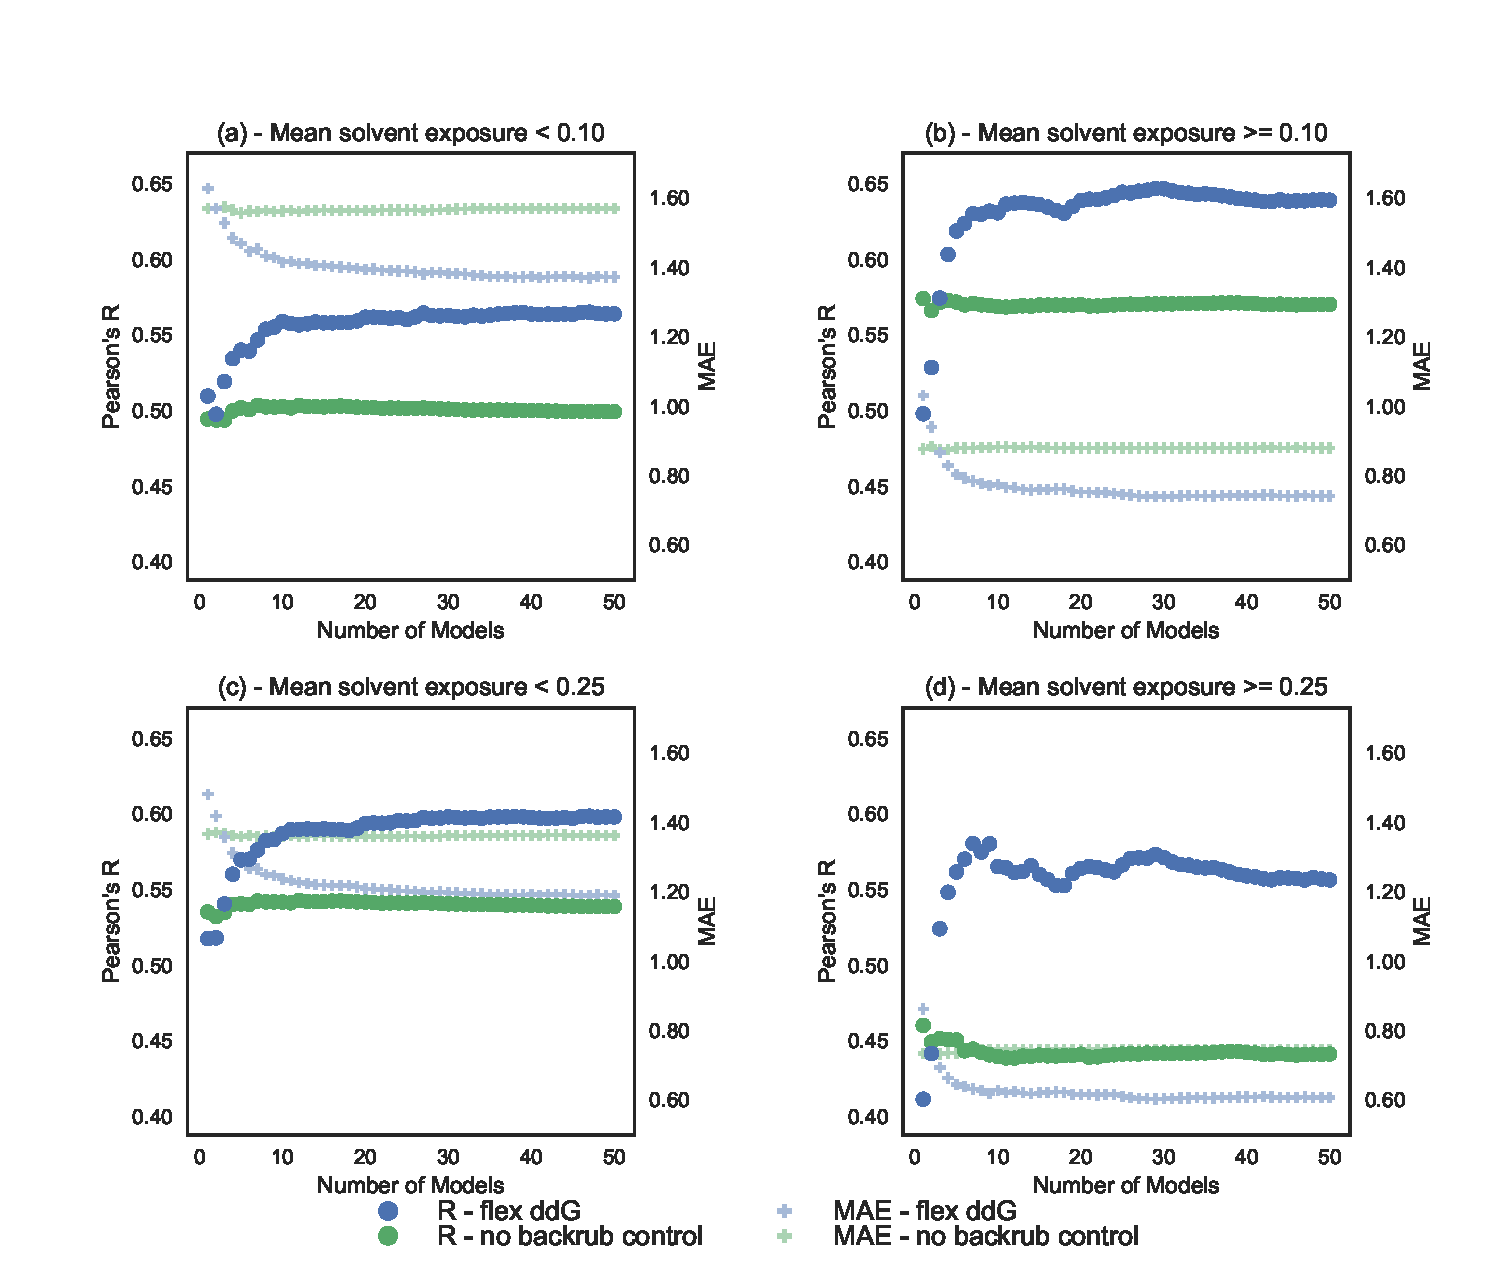
\includegraphics[width=\textwidth,keepaspectratio]{structs-v-corr-id-zemu-12-60000-rscript-simplified-t14-burial.pdf}
  \caption[]{
    Correlation (Pearson's R, left y-axis) and MAE (Mean Absolute Error, right y-axis) vs. number of averaged models (x-axis), on the complete ZEMu set, and subsets. This plot is analogous to \cref{fig:structs-v-corr-WildTypeComplex-zemu-12-60000-rscript-simplified-t14} in the main manuscript, except that the models used for averaging are not sorted by score.
    Pearson's R is shown as circles, and MAE as faded plusses.
Predictions generated with the Flex ddG protocol are shown in blue.
Predictions generated with the no backrub control protocol are shown in green.
    A selection of key data underlying this figure can be found in \cref{tab:structs-v-corr-id-zemu-12-60000-rscript-simplified-t14-burial-underlying-data}. Flex ddG is run with 35000 backrub steps.
    Structures are not sorted, and are randomly added to the ensemble. 
    (a) Mean burial score < 0.10 (n = 436)
    (b) Mean burial score >= 0.10 (n = 804)
    (c) Mean burial score < 0.25 (n = 758)
    (d) Mean burial score >= 0.25 (n = 482).
  } \label{fig:structs-v-corr-id-zemu-12-60000-rscript-simplified-t14-burial}
\end{figure}
